%%%%%%%%%%%%%%%%%%%%%%%%%%%%%%%%%%%%%%%%%
% Simple Sectioned Essay Temhttps://www.youtube.com/plate
% LaTeX Template
%
% This template has been downloaded from:
% http://www.latextemplates.com
%
% Note:
% The \lipsum[#] commands throughout this template generate dummy text
% to fill the template out. These commands should all be removed when 
% writing essay content.
%
%%%%%%%%%%%%%%%%%%%%%%%%%%%%%%%%%%%%%%%%%

%----------------------------------------------------------------------------------------
%	PACKAGES AND OTHER DOCUMENT CONFIGURATIONS
%----------------------------------------------------------------------------------------

\documentclass[10pt,twoside]{report} % Default font size is 12pt, it can be changed here
\usepackage{inputenc}
\raggedbottom
\usepackage{pdflscape}
%%%% PAGE FORMAT STUFF %%%%%
\usepackage[superscript,biblabel]{cite}
\usepackage[a4paper,width=150mm,top=25mm,bottom=25mm]{geometry} % Set the page size to be A4 as opposed to the default US Letter
%\addtolength{\oddsidemargin}{-0.25in}
%\addtolength{\evensidemargin}{-0.25in}
%\addtolength{\textwidth}{0.5in}
%\addtolength{\topmargin}{-.5in}
%\addtolength{\textheight}{1.5in}

%  HEADERS ON PAGE 
\usepackage{dsfont}
\usepackage{lscape}
\usepackage{dsfont}
\usepackage{fancyhdr}
\pagestyle{fancy}
\fancyhead{}
\fancyhead[RO,LE]{Supplementary Information}
\fancyfoot{}
\fancyfoot[LE,RO]{}
\fancyfoot[CO,CE]{\thepage}
\fancyfoot[RE]{}
\renewcommand{\headrulewidth}{0.2pt}
\renewcommand{\footrulewidth}{0.2pt}
\usepackage{booktabs}
\usepackage[]{algorithm2e}

\usepackage{appendix}

%%% CUSTOM CHAPTER WRITING %%%%%
\usepackage{titlesec}
\titleformat{\chapter}{\normalfont\huge\bf}{\thechapter.}{20pt}{\huge\bf}
\usepackage{footnote}
\usepackage{lscape}
\usepackage{amsmath}

%%%% TABLE STUFFFF %%%%%%%
\usepackage{longtable}
\makesavenoteenv{tabular}
\usepackage{multicol}
\usepackage{multirow}
\usepackage[labelfont=bf]{caption}
\usepackage{enumitem}

%%GRAPHICS STUFFF %%%%%%
\usepackage{ graphicx} % Required for including pictures
\usepackage{ rotating}
\usepackage{url}
\usepackage{float} % Allows putting an [H] in \begin{figure} to specify the exact location of the figure
\usepackage{wrapfig} % Allows in-line images such as the example fish picture
%\usepackage[titletoc]{appendix}
\usepackage{caption}
\usepackage{subcaption}

%%%TIKZ STUFF %%%%%%
\usepackage{lipsum} % Used for inserting dummy 'Lorem ipsum' text into the template
\usepackage{tikz}   
\usepackage{tikz-3dplot}
\linespread{1.2} % Line spacing
  
    


%\setlength\parindent{0pt} % Uncomment to remove all indentation from paragraphs

%%% MATHS STUFFF %%%%%%
\usepackage{amsmath, bm}
\usepackage{amsfonts}
\usepackage{setspace}
\usepackage{array}
\usepackage{blindtext}
\usepackage{mathtools}
\usepackage{breqn}
\DeclarePairedDelimiter\ceil{\lceil}{\rceil}
\DeclarePairedDelimiter\floor{\lfloor}{\rfloor}

\begin{document}

%----------------------------------------------------------------------------------------
%	TITLE PAGE
%----------------------------------------------------------------------------------------


%\begin{figure}[t]
   % \centering
    %\includegraphics[scale=0.35]{./images/Logo_Unisi_2012.jpg}
%\end{figure}    


%\begin{abstract}
%\centering
%\end{abstract}
%----------------------------------------------------------------------------------------
%	TABLE OF CONTENTS
%----------------------------------------------------------------------------------------
\setcounter{secnumdepth}{2}

\setcounter{tocdepth}{2}

\newpage % Begins the essay on a new page instead of on the same page as the table of contents 

%----------------------------------------------------------------------------------------
%	INTRODUCTION
%----------------------------------------------------------------------------------------


%\title{Strain-specific age dependent seasonal SIR model for Influenza transmission}
%\author{by David Hodgson}

%\date{}

%\maketitle


%\tableofcontents



\chapter{ptmc package performance}

\section{Background}
\paragraph{}Mathematically modelling the propagation of infectious diseases often involves solving complex non-linear SIR-type models. The evolution of these models are dictated by parameters values which are often difficult to accurately estimate due to biases in existing studies or surveillance data, leading to uncertainty in their estimates. The desire to formally incorporate such parameter uncertainty in epidemic models naturally leads to the use of Bayesian inference. However, combining Bayesian inference with complex non-linear systems forms intractable integrals which require Markov Chain Monte Carlo (MCMC) methods to solve. Given the rich, dense literature on MCMC samplers, it is often not clear which MCMC sampler is best to use (i.e. provides convincing convergence over a small time frame) for SIR-type infectious diseases models. 

\paragraph{}This analysis explores this issue, by comparing several popular MCMC samplers with a promising population-based MCMC sampler (parallel tempering), to sample from the posterior distribution for parameters in an age- and exposure-stratified epidemic model for Respiratory Syncytial Virus. The package finds that the population based parallel tempering MCMC sampler is significantly quicker and has improved mixing compared to popular MCMC samplers in existing packages. Therefore it is encouraged that mathematical modellers who require MCMC to calibrate epidemic models to use parallel tempering or explore similar population based samplers to ensure quick and convincing convergence. 

\section{Methods}
\subsection{Description of epidemic model}
\paragraph{}I modelled the number of individuals in six different epidemiological states, $S_0$, $I_0$, $R_0$, $S_1$, $I_1$, and $R_0$, where $S$, $I$, and $R$ refer to susceptible, infectious and recovered individuals respectively. The subscript $0$ relates to primary infection, and subscript $1$ refers to secondary and subsequent infections. On average, the infectious period lasts for $1/\gamma$ days and the duration of immunity lasts $1/\omega$ days. The epidemiological states are stratified into two different age groups (0--2 years, and 2+ years), denoted by superscript $a$. To ensure the population of each age group remains constant, I assume that $\mu = 1861$ live births occur each day into the 0-2 years age group and that the same number of persons die each day from the 2 years and older group. The rate at which individuals acquire infection, $\lambda^a_i$ depends on contacts between age groups and the number infectious persons in each age group. Thus, the RSV epidemic model is specified in a continuous time system for age group $a$ is given by:

\begin{equation}
\label{eq:1}
\footnotesize\renewcommand{\arraystretch}{1.5}
\begin{array}{r c l l l }
\frac{dS_0^{a}}{dt} & = &  \overbrace{\mu \mathds{1}_1(a) - \lambda^aS_0^{a}\;\;\;\;\;\;\;}^{\text{Transmission terms}}                                                                                                             & \overbrace{- \eta^{a} S_0^{a} + \eta^{a-1}S_0^{a-1}}^{\text{Ageing terms}}       \\
\frac{dI_0^{a}}{dt} & = & \lambda^aS_0^{a} - \gamma I_0^{a} & - \eta^{a} I_0^{a} + \eta^{a-1}I_0^{a-1} \\
\frac{dR_0^{a}}{dt} & = & \gamma I_0^{a} - \omega R_0^{a} 	& - \eta^{a} R_0^{a} + \eta^{a-1}R_0^{a-1} \\

\frac{dS_1^{a}}{dt} & = & \omega R_0^{a} + \omega R_1^{a}   - \delta_1\lambda^aS_1^{a}& - \eta^{a} S_1^{a} + \eta^{a-1}S_1^{a-1}  \\
\frac{dI_1^{a}}{dt} & = & \delta_1\lambda^aS_1^{a} - \gamma I_1^{a} & - \eta^{a} I_1^{a} + \eta^{a-1}I_1^{a-1} \\
\frac{dR_1^{a}}{dt} & = & \gamma I_1^{a}  - \omega R_1^{a}& - \eta^{a} R_1^{a} + \eta^{a-1}R_1^{a-1} \\

\frac{dZ^{a}}{dt} & = &  \lambda^a_0S_0^{a} + \lambda^a_1S_1^{a}\\

\end{array}
\end{equation}

where $\mathds{1}_1(a)$ is the indicator function (non-zero at $a=1$), $\eta^a$ is the rate of ageing from age group $a$ to age group $a+1$ (with $\eta^0 = 0$), and $\lambda^a(t)$ is the force of infection for age group $a$ given by 

\begin{equation}
\label{eq:2}
\lambda_i^a = \sum_{b=1}^2c^{a,b}\frac{I_0^b+I_1^b}{N^b}
\end{equation}

where $N^b$ is the population of age group $b$, $\delta_1$, is the relative susceptibility of the population to RSV infection after being infected, and $c^{a,b}$ is the number of daily contacts made between age group $a$ and $b$, estimated from the POLYMOD study. 
 
 he cumulative number of infections in age group $a$ is given by $Z^a$, so the number of new infections $z_w^a$ per week $w$ in age group $a$ can be calculated:
 
 \begin{equation}
 \left. \frac{dZ^a(t)}{dt}\right|_{7(w-1)}^{7w} = z_w^a
 \end{equation}



\subsection{Likelihood}

The data, $x$, used the calibrate the model is the number of weekly ($w$) confirmed positive RSV samples per age group ($a$) from the Respiratory DataMart System (RDMS) at PHE between July 2010 and June 2017. This data is patient sensitive so cannot be shared publicly. In the likelihood I assume that the number of confirmed positive RSV samples per age group and week ($x_w^a$) is the realisation of the random variable $X_w^a$,

\begin{equation}
X_w^a \sim \text{Bin}\left(z_w^a, \epsilon^a\right)
\end{equation}

where $\epsilon^a$ is the probability that someone with RSV is correctly identified in the RDMS dataset. By representing the set of all parameters to be fitted in the model as 

$$\Psi = \{\gamma, \omega, \delta_1, \alpha ,a, b, \phi, \psi, I_1, I_2, I_3, \epsilon^1, \epsilon^2\}$$

where $I_1, I_2, I_3$ are seeding parameters at $t=0$ as defined in \textbf{Table~\ref{tab:1}} the likelihood calcualted through:

\begin{equation}
\label{eq6}
\mathcal{L}(x, \Psi) = \prod_{t=1}^{52*7}\prod_{a=1}^2 \mathcal{L}(x_w^{a}; \Psi) = \prod_{t=1}^{52*7}\prod_{a=1}^2 \binom{z^a_w}{x^a_w}(\epsilon^a)^{x^a_w}(1-\epsilon^a)^{z^a_w-x^a_w}
\end{equation}


\subsection{Prior distributions}

A summary of all the model parameters with their prior distributions are contained in \textbf{Table~\ref{tab:1}}. In implementation the parameters are logit-transformed.

\begin{table}[H]
\renewcommand{\arraystretch}{1.5}
\centering\footnotesize
\begin{tabular}{ p{0.04\textwidth} p{0.50\textwidth} p{0.25\textwidth}p{0.1\textwidth}}%\centering\small35

& \textbf{Parameter} & \textbf{Prior distribution}  & \textbf{Source}\\ \hline
$1/\gamma$ & Duration of infection (days) &  $\mathcal{U}(2,20)$  &  \cite{}\\
$1/\omega$ & Duration of immunity (days) &  $\mathcal{U}(60,365)$  &  \cite{}\\
$\delta_1$ & Relative proportion of population susceptibility RSV after primary infection &  $\mathcal{U}(0,1)$ & ---   \\
$\alpha$ & Relative infectiousness of RSV after primary infection &  $\mathcal{U}(0,1)$ &   ---\\

\multicolumn{3}{l}{\textit{Parameters associated with transmission}}\\

$a$& Rate of infection   & $\mathcal{U}(0, 1)$  & ---\\ 
$b$& Amplitude &  $\mathcal{U}(0, 1)$ & ---\\ 
$\phi$& Peak transmission (offset) (days) &  $\mathcal{U}(100, 250)$ & RDMS\\ 
$\psi$& Width of seasonal peak&  $\mathcal{U}(0, 36.5)$ & ---\\ 

\multicolumn{3}{l}{\textit{Initial parameters (at $t=0$) }}\\

$I_1$ & Initial proportion infected RSV & $\mathcal{U}(0,1)$  &  ---\\ 
$I_2$ & Initial proportion recovered from RSV & $\mathcal{U}(0,1)$  &  ---\\ 
$1/I_3$ & Average duration between infections (years) & $\mathcal{U}(1,4)$  &  ---\\ 

\multicolumn{3}{l}{\textit{Detection rates}}\\

$\epsilon^1$ & 0--2 years  & $\mathcal{U}(0.0, 0.01)$  &  ---\\ 
$\epsilon^2$ & 2+ years  & $\mathcal{U}(0.0, 0.01)$  &  ---\\ 

\hline
\end{tabular}
  \caption{Prior distributions of the parameters in the mathematical model. \label{tab:1}}
\end{table}

\subsection{MCMC samplers}

\subsubsection{Overview of sampling methods} 
\paragraph{}To sample values from the posterior distribution of the fitted parameters, we use Bayes rule

\begin{equation}
\pi(\Psi) = p(D|\Psi) \propto \mathcal{L}(x, \Psi)p(\Psi)
\end{equation}

which simplifies the problem to sampling from the previously-defined likelihood and priors. To generate the random samples we use four different types of MCMC samplers; a normal Metropolis-Hastings (MH), an adaptive Metropolis-Hastings (AMH), a Differential Evolution (DE) and a parallel tempering (PT). For the MH algorithm the proposal distribution assumes no covariance between parameters. The AMH algorithm in which the proposal distribution is a normal distribution with a covariance matrix estimated from previous values in the chain. The DE algorithm is one in which XXXX. The PT algorithm runs various chains which have an likelihood which is altered so that some (hotter) chains accept many proposals and other (colder) chains are similar to an unaltered likelihood. 


\subsubsection{Implementation} 
The MH, AMH, and DE samplers are implemented via the BayesianTools R package. Explicit details about their implementation is best explained within the documentation. These three samplers for 1,000,000 steps with thinning occurring every 10th step. The PT sampler is implemented via the ptmc R package () and is run for 100,000 steps with a temperature ladder of 10 chains per run with thinning every 10th step (only the coldest chain is used to calculate the posterior distribution). The burn in is half of the total run time and each of the four samplers and each are ran ten times so that convergence via Gelman-Rubin statistics and manual inspection of trace plots can be performed. An R Markdown file with all code used for this analysis can be found XX. 

\newpage
\section{Results}
The trace plots for the log(-LL) for 10 runs of each of the four MCMC samplers are given below. 

\subsection{MH}

For the standard random-walk Metropolis-Hastings algorithm, only one of the ten chains appears to reach the convergent state after one millions samples. 

\begin{figure}[H] % Inline image example
\centering
    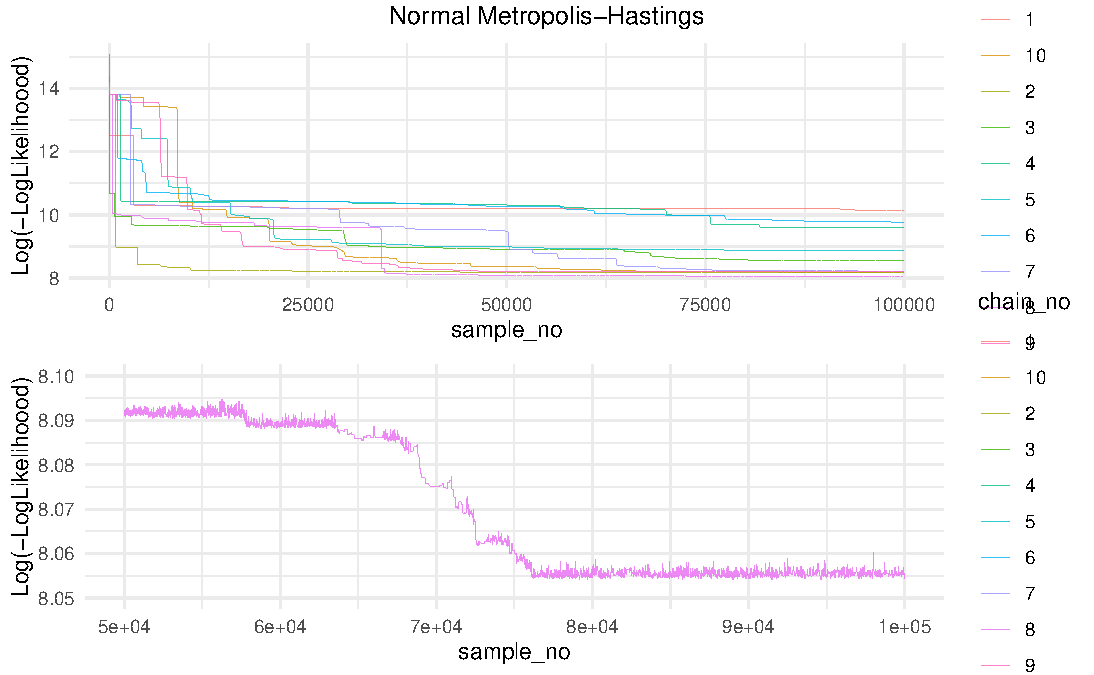
\includegraphics[width=1.0\textwidth]{../figs/llogMH.pdf}
  \caption{\label{fig:1}}  
\end{figure}

\subsection{AM}

For the adaptive Metropolis-Hastings algorithm, only two of the ten chains appears to reach the convergent state after one millions samples. 

\begin{figure}[H] % Inline image example
\centering
    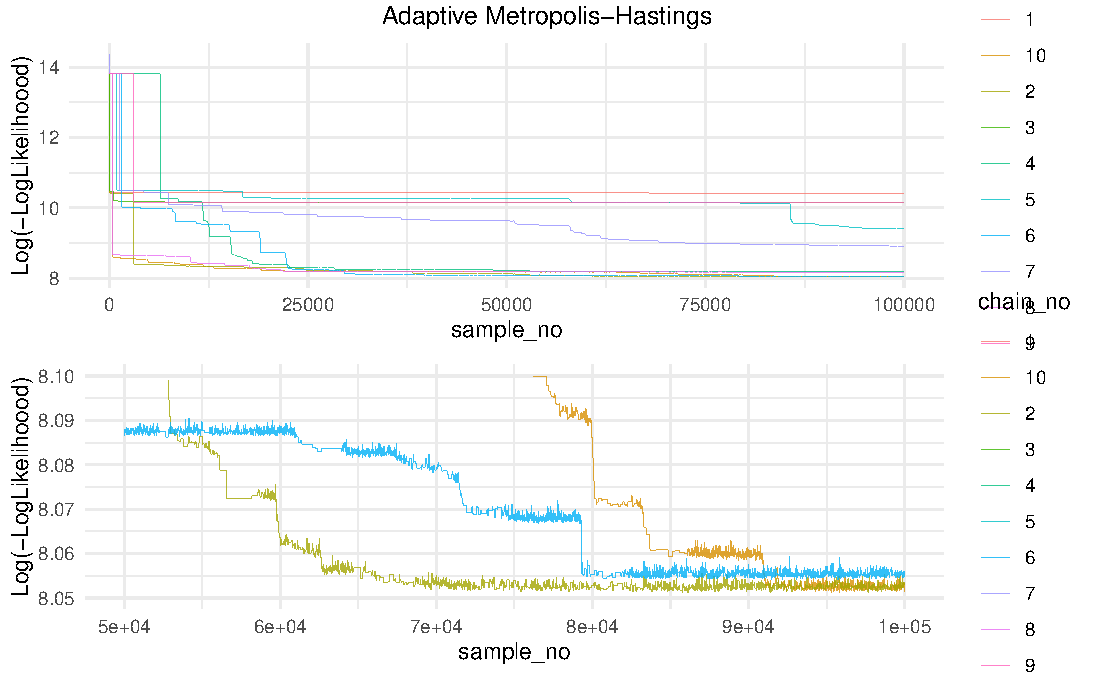
\includegraphics[width=1.0\textwidth]{../figs/llogAM.pdf}
  \caption{\label{fig:2}}  
\end{figure}

\subsection{DE}
For the adaptive Metropolis-Hastings algorithm, only one of the ten chains appears to reach the convergent state after one millions samples. 

\begin{figure}[H] % Inline image example
\centering
    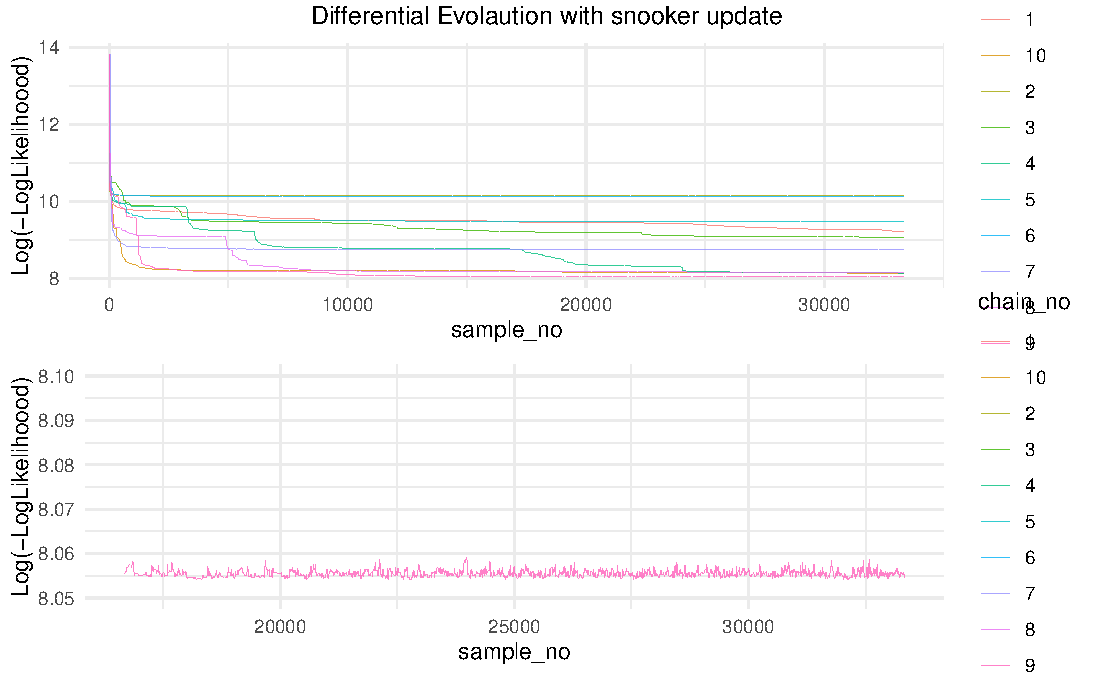
\includegraphics[width=1.0\textwidth]{../figs/llogDE.pdf}
  \caption{\label{fig:3}}  
\end{figure}

\subsection{PT}

or the adaptive Metropolis-Hastings algorithm, all ten chains appear to reach the convergent state after 100,000 samples. 

\begin{figure}[H] % Inline image example
\centering
    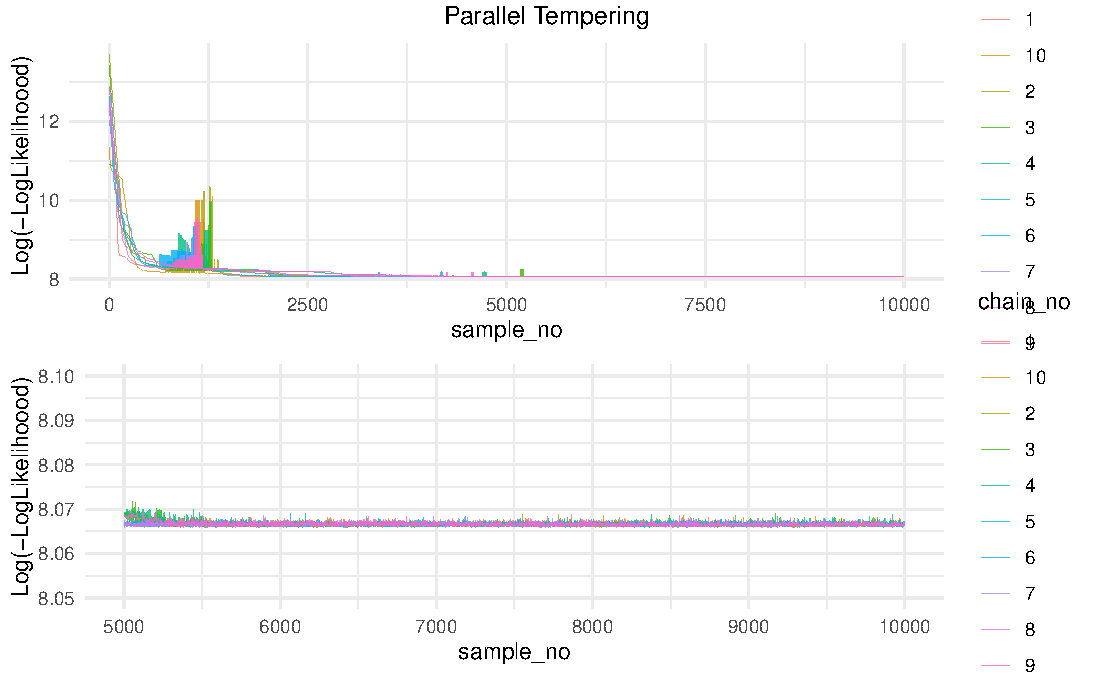
\includegraphics[width=1.0\textwidth]{../figs/llogPT.pdf}
  \caption{\label{fig:4}}  
\end{figure}

\begin{figure}[h] % Inline image example
\centering
    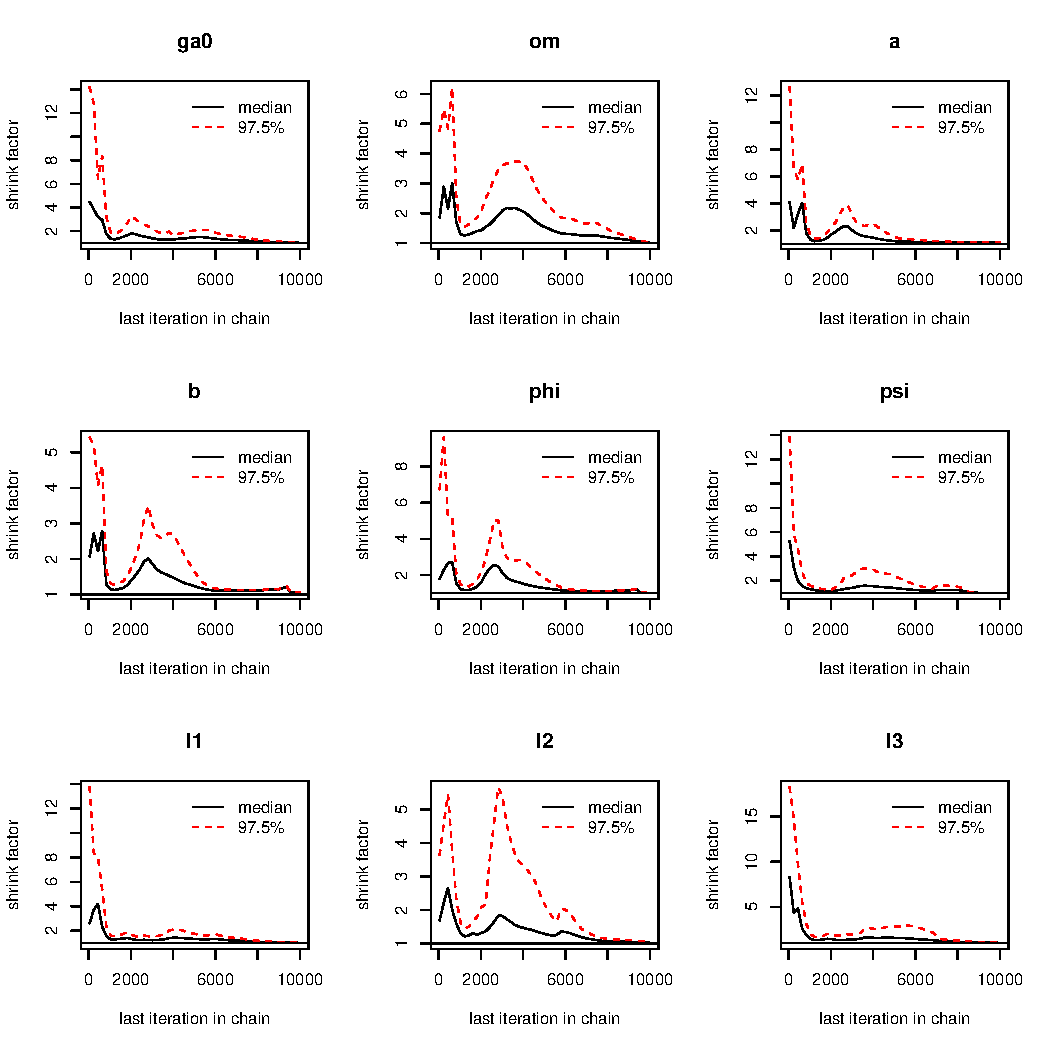
\includegraphics[width=1.0\textwidth]{../figs/convPT.pdf}
  \caption{\label{fig:5}}  
\end{figure}


\section{Discussion}
\paragraph{}The MCMC samplers are run for a fixed duration to see which provides the most reassuring convergence in a given space of time. The parallel tempering has the most convincing convergence compare to the other 3 samplers, with all 10 of the chains converging in contrast to the other MCMC samplers. The multivariate potential scale reduction factor is 1.03 and less than 1.08 for all the fitted parameters for the parallel tempering, suggesting convergence has occurs. 

\paragraph{}It is encouraged that future epidemic models will use the parallel tempering MCMC sampler (through the ptmc R package) to sample from posterior distributions. Using such pre-built algorithms will assuage mathematical modellers concerns surrounding convergences of epidemic models, allowing more time for analysis more relevant to policy makers (i.e. impact of intervention programmes or cost-effectiveness analysis) to be performed. 


%----------------------------------------------------------------------------------------
%	BIBLIOGRAPHY
%----------------------------------------------------------------------------------------

\bibliographystyle{vancouver}
\bibliography{ref}





%%%%%%%%%%%%%%%%%%%%
%%% IMAGE %%%%%%%%%%%%%
%%%%%%%%%%%%%%%%%%%%
%\begin{figure}[h] % Inline image example
%\centering
 %   \includegraphics[width=0.8\textwidth]{Nerve}
   % \vspace{-15pt}
  %\caption{\label{fig:a}}  
%\end{figure}
%%%%%%%%%%%%%%%%%%%

%%%%%%%%%%%%%%%%%%%%
%%% IMAGE WRAP IMAGES %%%%%
%%%%%%%%%%%%%%%%%%%%
%\begin{wrapfigure}{r}{0.5\textwidth} % Inline image example
%  \begin{center}
  %\vspace{-20pt}
    %\includegraphics[width=0.5\textwidth]{axon1}
 % \end{center}
   % \vspace{-15pt}
  %\caption{ \label{fig:b}}
%\end{wrapfigure}

%%%%%%%%%%%%%%%%%%%%
%%% IMAGE SUBIMAGES %%%%%%
%%%%%%%%%%%%%%%%%%%
%\begin{figure}[h] % Inline image example
%\centering
%	\begin{subfigure}[b]{0.45\textwidth}
%	    \includegraphics[width=\textwidth]{LINK}
%	    \vspace{-15pt}
%		\caption{}
%		\label{}
  %\end{subfigure}
 % \begin{subfigure}[b]{0.45\textwidth}
  %  \includegraphics[width=\textwidth]{LINK}
  %  \vspace{-15pt}
%\caption{}
%\label{}
  %\end{subfigure}
    %\caption{\label{}  }
%\end{figure}




%Users/davidhodgson/Dropbox/PhD/phd_thesis/c3modeldesc/main_C/
%----------------------------------------------------------------------------------------

\end{document}%%